
%(BEGIN_QUESTION)
% Copyright 2006, Tony R. Kuphaldt, released under the Creative Commons Attribution License (v 1.0)
% This means you may do almost anything with this work of mine, so long as you give me proper credit

Et ohmmeter viser en resistans på 8,5 k$\Omega$ når det kobles mellom to metallplater nedsenket i en vannprøve. Metallplatene er hver 2 centimeter ganger 2 centimeter, og er adskilt med en avstand på 10 centimeter:

$$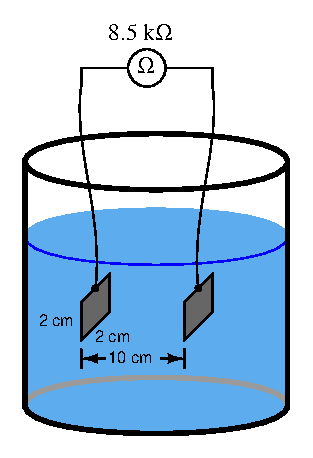
\includegraphics[width=15.5cm]{i00907x01.eps}$$

Beregn den spesifikke ledningsevnen til dette vannet, uttrykt i mikrosiemens per centimeter ($\mu$S/cm):

\vskip 10pt

Spesifikk ledningsevne = \underbar{\hskip 50pt} $\mu$S/cm

\underbar{file i00907}
%(END_QUESTION)





%(BEGIN_ANSWER)

Spesifikk ledningsevne = \underbar{\bf 294.12} $\mu$S/cm

%(END_ANSWER)





%(BEGIN_NOTES)

%INDEX% Measurement, analytical: conductivity

%(END_NOTES)

